%
%  Chris Thoma
%
\documentclass[12pt,fullpage]{article}
\usepackage{fullpage}
\usepackage{psfrag}                                          % LaTeX graphics tool
\usepackage{pslatex}                                         % avoids the default cmr font
\usepackage{graphicx}                                        % graphics package 
\usepackage{hyperref}
\usepackage{color}

\begin{document}

\noindent
{\bf Exponential power distribution} (from \color{blue}\url{http://www.math.wm.edu/~leemis/chart/UDR/UDR.html}\color{black})

\noindent
The shorthand $X \sim \hbox{exponential power}(\lambda, \, \kappa)$ is used to indicate that the
random variable~$X$ has the exponential power distribution with positive scale parameter $\lambda$ and positive shape parameter $\kappa$.
An exponential power random variable $X$ has probability density function 
$$
f(x) = \left(e ^ {1 - e ^ {\kern 0.04 em \lambda \kern 0.08 em x ^ \kappa}} \right) e ^ {\kern 0.08 em \lambda \kern 0.08 em x ^ \kappa} \lambda \kappa \kern 0.08 em x ^ {\kappa - 1} \qquad \qquad x > 0.
$$
The exponential power distribution is one of the few two-parameter distributions that
can achieve a bathtub-shaped hazard function.
The probability density function for three different parameter settings is illustrated below.
{\begin{figure}[h!]
\begin{center}
\psfrag{lab1}{$\lambda \kern -0.08 em = \kern -0.08 em  1, \kappa \kern -0.08 em  = \kern -0.08 em  1$}
\psfrag{lab2}{$\lambda \kern -0.08 em  = \kern -0.08 em  2, \kappa \kern -0.08 em  = \kern -0.08 em  1$}
\psfrag{lab3}{$\lambda \kern -0.08 em  = \kern -0.08 em  1, \kappa \kern -0.08 em  = \kern -0.08 em  2$}
\psfrag{labx}{$x$}
\psfrag{labf}{$f(x)$}
\includegraphics[width=3.2in]{ExponentialpowerPlot.ps}
\end{center}
\end{figure}}\\
The cumulative distribution function on
the support of $X$ is
$$
F(x) = P(X \le x) = 1 -  e ^ {1 - e ^ {\kern 0.04 em \lambda \kern 0.04 em x ^ {\kern 0.04em \kappa}}} \qquad \qquad x > 0.
$$
The survivor function on the support of $X$ is
$$
S(x) = P(X \ge x) = e ^ {1 - e ^ {\kern 0.04 em \lambda \kern 0.04 em x ^ {\kern 0.04em \kappa}}} \qquad \qquad x > 0.
$$
The hazard function on the support of $X$ is
$$
h(x) = \frac{f(x)}{S(x)} = e ^ {\lambda \kern 0.04 em x ^ {\kern 0.04 em\kappa}} \lambda \kappa \kern 0.08 em x ^ {\kappa - 1} \qquad \qquad x > 0.
$$
The cumulative hazard function on the support of $X$ is
$$
H(x) = - \ln S(x) =  e ^ {\lambda x ^ {\kern 0.04 em\kappa}} - 1 \qquad \qquad x > 0.
$$
The inverse distribution function of $X$ is
$$
F ^ {-1}(u) = \left[ \frac{1}{\lambda} \ln \left( 1 -  \ln(1-u) \right) \right] ^ {1/ \kappa} \qquad \qquad 0 < u < 1.
$$
The median of $X$ is 
$$
F ^ {-1}(1/2) = (\lambda \ln(1-\ln(1/2))) ^ {-1/ \kappa}.
$$
The moment generating function of $X$ is
$$
M(t) = E\left[ e ^ {\kern 0.04em tX} \right] = \displaystyle \int_0 ^\infty \lambda \kappa \kern 0.08 em x ^ {\kappa - 1}
e ^ {tx + 1 + \lambda \kern 0.04 em x ^ \kappa - e ^ {(\lambda \kern 0.04 em x ^ \kappa)}} \, dx.
$$
The characteristic function of $X$ is
$$
\phi(t) = E\left[ e ^ {itX} \right] =  \displaystyle \int_0 ^\infty \lambda \kappa \kern 0.08 em x ^ {\kappa - 1} e ^
{itx + 1 + \lambda \kern 0.04 em x ^ \kappa - e ^ {(\lambda \kern 0.04 em x ^ \kappa)}} \, dx.
$$
The population mean, variance, skewness, and kurtosis of $X$ are mathematically intractable.\\

\vspace{0.1in}
%\newpage
\noindent
{\bf APPL verification:}
The APPL statements
\begin{verbatim}
X := ExponentialPowerRV(lambda, kappa);
CDF(X);
SF(X);
HF(X);
IDF(X);
MGF(X);
\end{verbatim}
verify the cumulative distribution function, hazard function, inverse distribution function, and moment generating function.
\end{document}
